% vim: spell spelllang=en_gb
\chapter{Literature Review}

The massive and accessible volume of data that social media produces has attracted the attention of
many researchers as a valuable data source for their research topic; however, collecting and
processing data of this nature pose many challenges to extracting useful information. This section
mentions what other researchers focusing on disaster management topics did to address these
challenges while using Twitter; it also discusses the different approaches used for identifying
relevant tweets, extracting geographical location from them, making text analysis on the text, and visualizing the results.

\section{Data Collection} 

Twitter's \ac{API} enables developers to retrieve historical tweets using
queries that are made of operators to match a variety of tweet attributes, such as a specific
keyword, having a geotag provided by the user who created the tweet, and the language classified by
Twitter. Users generate around 500-700 million tweets a day \cite{inproceedings}, making it
necessary to limit the number of tweets to fetch using the \ac{API} to reduce computational power and
downtime. \citeauth{fengExtractionPluvialFlood2018} only fetches geotagged tweets and then filters
necessary
them using 45 keywords in 7 languages; this approach filters out a big chunk of relevant tweets
since 1\% of tweets are geotagged \cite{middletonRealTimeCrisisMapping2014}. A better approach is to
fetch tweets using keywords related to the topic of interest in different languages.
\citeauth{debruijnGlobalDatabaseHistoric2019b} uses over 40 keywords associated with floods in 11
major languages in the query to fetch tweets.

In addition to using textual data, some researchers use other types of data to enhance their
pipelines. Some tweets contain media attachments, such as images and videos that are potential
visual information for the concerned research topic
\cite{alamFloodDetectionTwitter2020}\cite{saidFloodsDetectionTwitter2020}\cite{ningPrototypingSocialMedia2020};
search engines are another resourceful source for images as well
\cite{fengExtractionPluvialFlood2018}. When it comes to flooding events, hydrological information
can be a valuable source of information that can be extracted from a global precipitation dataset
based on tweets' time stamps and location in the text
\cite{debruijnImprovingClassificationFlood2020}.
\citeauth{barkerDevelopmentNationalscaleRealtime2019} use Environment Agency flood-monitoring
\ac{API}\footnote{https://environment.data.gov.uk/flood-monitoring/doc/reference\#flood-warnings} to
get river gauge levels and flood warnings to identify at-risk flooding areas.

Processing text is a crucial part of any \ac{NLP} pipeline to train an effective classifier.
Research requires that the corpus is in multiple languages, so translating the text to one language
(most likely English) is needed if the classifier can not handle multilingual data
\cite{singhEventClassificationLocation2019}. One of the most common text-processing tasks is
removing unnecessary terms such as stopwords, Uniform Resource Locator URLs, numbers, and
punctuation marks. User mentions in tweets don't provide useful information, so pipelines often
remove or replace them with a generic term such as
``@user''\cite{debruijnImprovingClassificationFlood2020}. The location of the flood event is an
important piece of information that is extracted from a term in the tweet, making it a potential
target that includes biases in the dataset by overusing it;
\citeauth{debruijnImprovingClassificationFlood2020} replaces these terms by the country name that
the location is located in; on the other hand,
\citeauth{petersenIdentificationExplorationExtreme2021} replace the terms by the word ``place'' if
they get mentioned more than 0.5\% of the size of the data set. Another way to improve the
performance of the classifier is to group the terms by converting them to lower-case and
transforming them to their lexeme or word stem by lemmatisation or stemming respectively.

Some tweets are noisy or redundant, making them a target for filtering out. Retweets are identical
to other tweets without additional context making them unneeded. Spam bots generate similar tweets
for malicious reasons, such as spreading false content to manipulate the public; other reasons could
be for utility reasons, such as creating a feed for users to check updates. These tweets introduce
noise to the dataset that gets reduced by removing duplicate tweets.
\citeauth{debruijnGlobalDatabaseHistoric2019b} only considers one tweet from each user in the last
14 days mentioning a specific region; they also remove tweets containing more than five consecutive
words that match with those in another tweet among the previous 100 talking about a location.
\citeauth{singhEventClassificationLocation2019} approaches this problem by only extracting tweets
created from mobile phones and only considers tweets from users who have $\text{followers} /
\text{following} < 1$.

\section{Text Classification}
Identifying disaster events using social media requires a classifier to determine the relevant data.
Textual data containing terms related to a disaster doesn't mean that it discusses a disastrous
event since words such as ``flood'' can be used figuratively in sentences (e.g., a flood of joy). A
binary classifier labelling the data with ``on-topic'' and ``off-topic'' labels is needed to filter
out irrelevant content.

Most classifiers use supervised \ac{ML} algorithms requiring labelled data for training. A
straightforward approach is to manually label a sample of the tweets
\cite{debruijnGlobalDatabaseHistoric2019b}\cite{barkerDevelopmentNationalscaleRealtime2019}.
\citeauth{petersenIdentificationExplorationExtreme2021} use Crisilext6
\cite{olteanuCrisisLexLexiconCollecting2014}, a crowdsource labelled tweets, for training their
classifiers that get evaluated on 88 million unlabelled tweets containing flood-related terms
\cite{DVN/T3ZFMR_2019}. \citeauth{fengExtractionPluvialFlood2018} automatically label the tweets by
checking if there is rainfall during the provided time and city location by using a weather
\ac{API}\footnote{https://www.wunderground.com/weather/api/d/docs}; if there's a rainfall, the tweet
is labelled positive, negative otherwise.

A classifier needs a numerical representation of the textual data for training. Text is often
represented in a real-valued vector by encoding words and their context. There are different word
embedding techniques, such as \ac{TF-IDF} \cite{enwiki:1123031029} that reflect how important a word
is to a document in a corpus. Word2vec \cite{mikolovEfficientEstimationWord2013} and its extension
doc2Vec \cite{leDistributedRepresentationsSentences2014} are other word embedding techniques that
capture the semantic and syntactic qualities of words via a vector space with several hundred
dimensions, where each unique word in the corpus gets assigned to a vector in the space.

There are different groups of \ac{ML} algorithms to classify data for varying data types. Supervised
algorithms are employed if the training data set is labelled; otherwise, a probabilistic approach
can be used by training a naive Bayes classifier on  labelled and unlabelled data
\cite{liDisasterResponseAided2018}. \citeauth{fengExtractionPluvialFlood2018} use naive Bayes,
random forest, logistic regression, \ac{SVM} (RBF Kernel), and \ac{SVM} (Linear Kernel) on labelled
data transformed using \ac{TF-IDF} with accuracies of 0.7109, 0.7582, 0.7705, 0.7712, and 0.7739,
respectively. \citeauth{petersenIdentificationExplorationExtreme2021} results are more promising,
where they train a logistic regression and random forest classifiers with 0.939 and 0.9253
accuracies, respectively. Deep learning approaches  generally outperform classical algorithms; one
example is \ac{CNN} trained on word embeddings for sentence classification.
\citeauth{fengExtractionPluvialFlood2018} and
\citeauth{petersenIdentificationExplorationExtreme2021} train a \ac{CNN} model on word2vec
embeddings with 0.7868 and 0.94611 accuracies, respectively.

Recently, transfer learning has been gaining popularity; it's the idea of transferring knowledge
acquired by solving one problem to other related problems. In the case of text classification,
\ac{RNN} is a class of artificial neural networks that process sequences of data using \ac{LSTM}
making it a suitable algorithm for \ac{NLP} tasks;
\citeauth{petersenIdentificationExplorationExtreme2021} fine-tunes the pre-trained \ac{ULMFit}
\cite{howardUniversalLanguageModel2018} with an accuracy of 0.9499. Models using transforms
architecture outperform \ac{RNN} in many \ac{NLP} tasks. One popular example is \ac{BERT}
\cite{devlinBERTPretrainingDeep2019}, a deep learning-based \ac{NLP} pre-training technique used by
generalized models by training on a massive dataset; afterwards, they are fine-tuned on a smaller
one for a specific task. \citeauth{alamFloodDetectionTwitter2020} uses a pre-trained \ac{BERT} model
that works on one language with an accuracy of 0.853, and
\citeauth{debruijnGlobalDatabaseHistoric2019b} uses a multilingual model with 0.8 F1-score.

Visual data such as images are usually classified using \ac{CNN} models by getting the results of
the models after removing the output layer to get a feature vector to train classifiers. These
models are pre-trained on massive datasets such as Imagenet
\cite{krizhevskyImageNetClassificationDeep2017} and places database
\cite{zhouLearningDeepFeatures2014}. \citeauth{fengExtractionPluvialFlood2018} use GoogLeNet
(Inception-V3 model) \cite{7780677} pre-trained on ImageNet to train multilayer perceptron, random
Forest, gradient boosted trees, and  xgboost with accuracies of 0.8907, 0.9133, 0.9252, and 0.9295,
respectively. \citeauth{ningPrototypingSocialMedia2020} uses VGGNet
\cite{simonyanVeryDeepConvolutional2015}, Inception V3, ResNet \cite{heDeepResidualLearning2015},
and DenseNet201 \cite{huangDenselyConnectedConvolutional2018} with 0.91 accuracy.

\section{Location Extraction}
Identifying the locations of disasters is helpful for the disaster management cycle. Social media
enables people to generate \ac{VGI}, which is more advantageous over the more expensive accuracy
testing by official agencies because contributors have unique local knowledge.  Detecting a
disastrous event and its location as soon as possible can reduce its impact on society
\cite{debruijnGlobalDatabaseHistoric2019b} by informing the citizens and the authority to prepare
for it. During the event, the rescue teams' task would be easier if they can locate the endangered
people \cite{singhEventClassificationLocation2019}. After the event wanes, assessing the most
impacted spots can enable the authority to make informed decisions on a recovery plan.

Users can assign an accessible property to their tweets, called ``geotag'' , a geographical
identification metadata. Adding ``has:geo'' to the query sent to the API will return geotagged
tweets with metadata about the location, such as a display name, geo polygon, and a geo lat-log
coordinate. The geotag is the most straightforward method to identify the locations 
\cite{fengExtractionPluvialFlood2018}, but unfortunately, only 1\% of the tweets are geotagged
\cite{middletonLocationExtractionSocial2018}, making it not include a massive amount of tweets
mentioning locations.

Locations can be extracted using toponyms, a place's name, in tweets' text by using geoparsing.
Geoparsing is a process of converting free-text descriptions of places
(such as ``twenty miles northeast of Jalalabad'') into unambiguous geographic identifiers. A toponym
can have more than one location candidate, such as ``Boston'', which is the name of several places,
including ``Boston, USA'' and ``Boston, UK''; this fact makes geoparsing tasks on a global scale
harder than local ones. \citeauth{debruijnGlobalDatabaseHistoric2019b} uses TAGGS
\citeauth{debruijnTAGGSGroupingTweets2017}, a geoparsing algorithm, to extract countries,
administrative areas, and settlements (i.e. cities, towns, and villages) mentioned within the tweets'
text on a global scale. The process includes toponym recognition and toponym resolution.  Toponym
recognition extracts the toponyms that refer to one or more locations using a gazetteer, a
geographical index, or a dictionary. Toponym resolution predicts the correct location for the
toponyms in several steps.A score is assigned to each possible location using metadata related to
the tweet, such as the user's timezone \& hometown, the tweet's coordinates, and mentions of nearby
locations. Then, calculate the average score of grouped tweets mentioning the same toponym within a
24-hour. Finally, assign the groups of tweets with the location that has the highest score.
\citeauth{petersenIdentificationExplorationExtreme2021} uses geotag property, geoparsing using
\ac{NER} on text, and user's profile location to extract toponyms. If the text contains two
toponyms, check if they are close with a distance threshold of 1500km, choose one of them randomly.
They use GeoPy\footnote{https://geopy.readthedocs.io/en/stable/} to assign geographical locations to
toponyms, a Python package that is a client for several popular geocoding web services (e.g.,
GoogleV3 and GeoNames). \citeauth{singhEventClassificationLocation2019} uses the fact that people
visit the same locations daily to generate a Markov chain model on historical tweets created by the
same user to locate them.
 
\section{Text Analysis}

Besides text classification and location extraction, other text analysis techniques extract
valuable information from text data. In the case of disasters, disaster managers can use social
media to get insights, such as how impactful an event is on society. They can visualize the results
to understand the situation and act accordingly. 

\citeauth{grunder-fahrerHowSocialMedia2018} extract multiple relevant pieces of information from
social media and present them to disaster managers via a searchable application. They extract the
following: topics using HDP-CRF algorithm \cite{tehHierarchicalBayesianNonparametric2010},
locations using Openstreetmap\footnote{https://www.openstreetmap.org/} location markers, time using
the social media meta data, and names of organizations using \ac{NER}. They present
the information using several interactive graphs such as pie charts, word clouds and line graphs.

Sentiment analysis is a popular text analysis technique that shows people's sentiments during an
event. \citeauth{luVisualizingSocialMedia2015} extract sentiment analysis from Twitter about the
Ebola virus using three different sentiment classifiers to measure the sentiment score of the tweet
depending on the majority of the votes. Also, they calculate the inconsistency between the
classifiers using an entropy measure \cite{argamon-engelsonCommitteeBasedSampleSelection1999}. The
positive and negative sentiments are each presented in a density map using solid blue and red
colours, respectively; the colour is blurred insread if the inconsistency score is above a certain
threshold. \citeauth{perinan-pascualAssessingImpactTweets2020} tries to extract the sentiment by
calculate three scores for the tweets: (1) the reliability of how much the tweet discusses a problem
during a hazard, (2) the impact of the tweet by using the user's activity and popularity as well as
how much influence the tweet is \cite{palIdentifyingTopicalAuthorities2011}, (3) and the impact of
the problem using the previous scores. They present the mean of the scores on a time frame basis on
a line graph.

\section{Visualization}
Visualization of the results of an \ac{NLP} pipeline is common practice for several reasons. The
massive and complex data can communicate the needed knowledge for different audiences to understand
the underlying situation and take action accordingly. The developers can use the visualization to
validate that the pipeline is working as intended. The authority can check the Spatio-temporal data
to identify places that have recurring floods and reinforce their infrastructure to prepare for
future flooding. Also, the plots make event detection and monitoring much faster and more
straightforward.

\citeauth{debruijnGlobalDatabaseHistoric2019b} uses historical and real-time data to show flooding
events on different levels (countries, administrative areas, and settlements). It is powered using a
JavaScript library, leaflet\footnote{https://leafletjs.com/}. The application, seen in figure
\ref{fig:global}, contains a map showing the flooding events with an adjustable timeline and a list
of tweets for the selected location.


\begin{figure}[H]
\begin{center}
  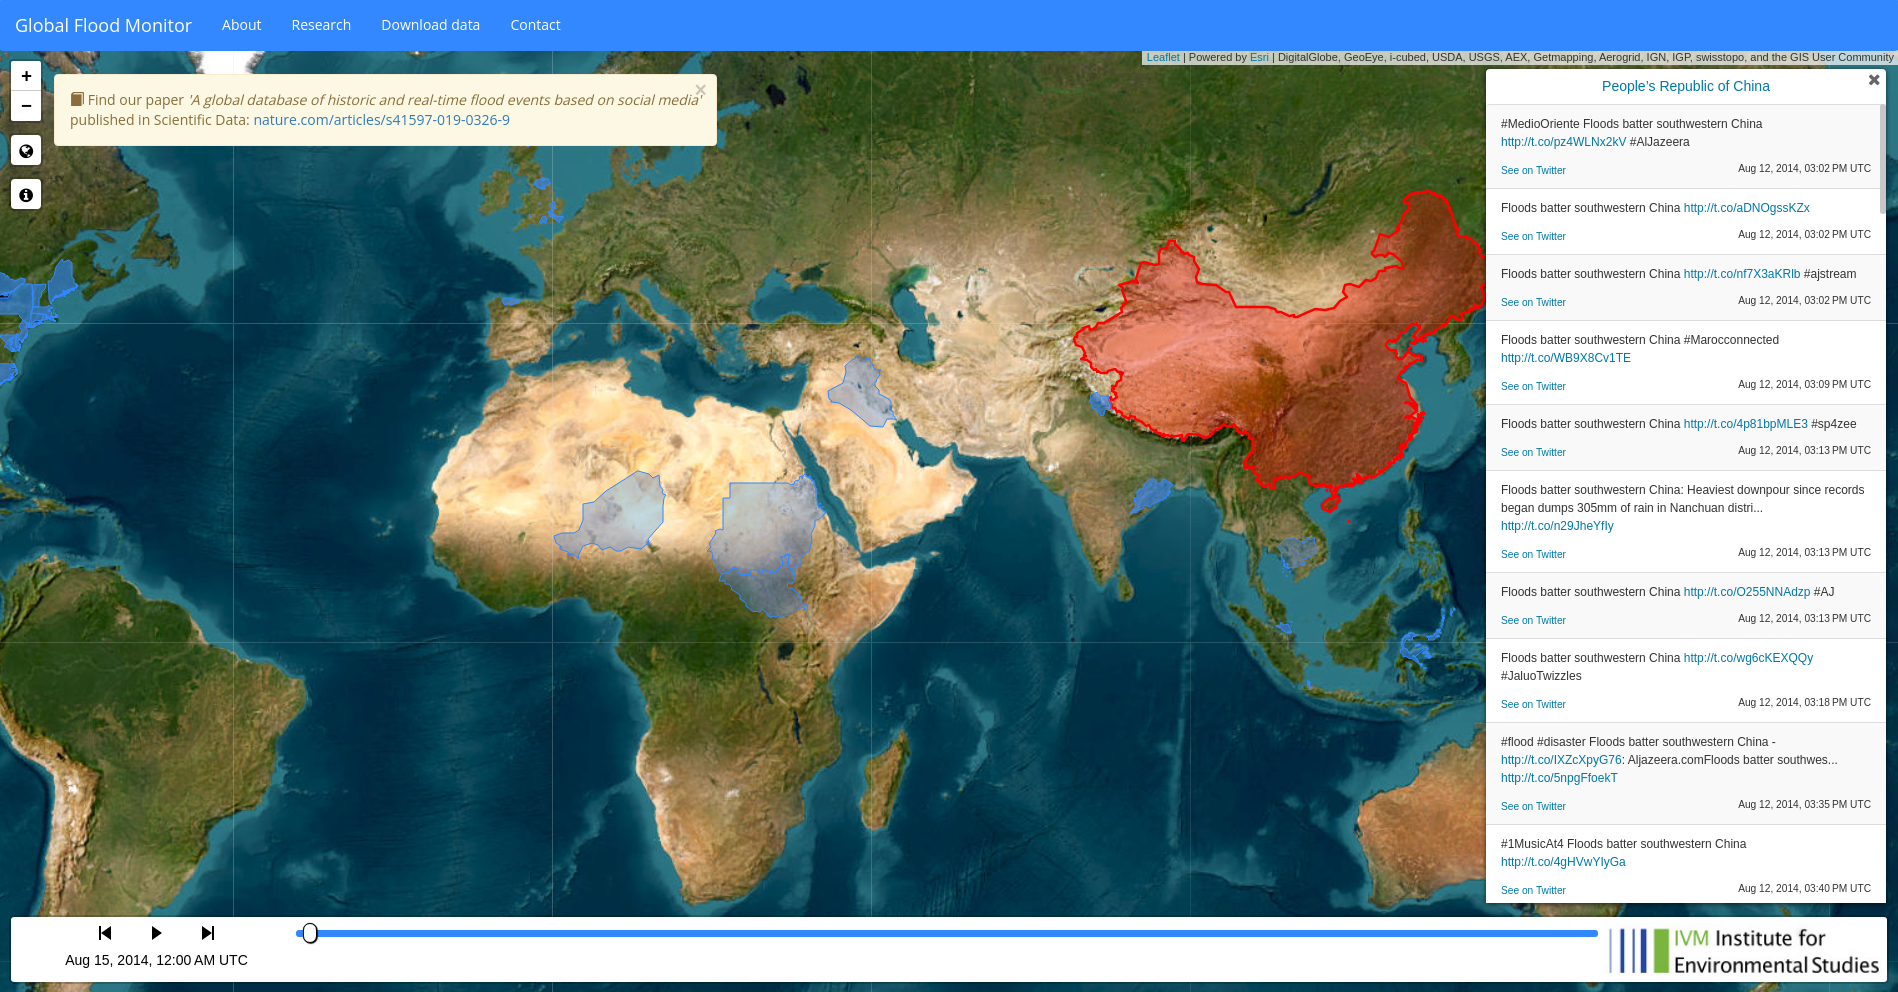
\includegraphics[width=\columnwidth]{images/global.png}
\end{center}
\caption{Global Flood Monitor application showing flood events}
\label{fig:global}
\end{figure}

\citeauth{petersenIdentificationExplorationExtreme2021} provide multiple plots with sophisticated
methods to configure the interface and filter the tweets. Their visualization is powered using the python
libraries, Plotly\footnote{https://plotly.com/python/} and Dash\footnote{https://dash.plotly.com/}.
The app, shown in figure \ref{fig:peter}, provides an interface to showcase the different aspects of the
data: spatial via a map, temporal via a histogram, and textual via a list of tweets and word cloud.
They use a scatter map to show the locations extracted from the tweets, where the colour of each
point represents the method used to identify the location. To resolve the problem of tweets
overlapping each other due to the discussion of the same location, the identical points are
spread by adding Gaussian noise to their coordinates points. As for representing the timestamps,
they use a histogram aggregated by each day with a time slider. Researchers can pinpoint repetitive
or interesting topics by navigating the word cloud to see the most frequent keywords or manually
navigating the list of tweets. The plots are interactive, where actions in one of them would
influence others. The data can be filtered in different ways: keywords in the text, the method used
to extract the location, tweet type (a retweet or not), a map, and a histogram. In addition, there is a
drop-down to change the map graph type and the algorithm used to classify the tweets.

\begin{figure}[H]
\begin{center}
  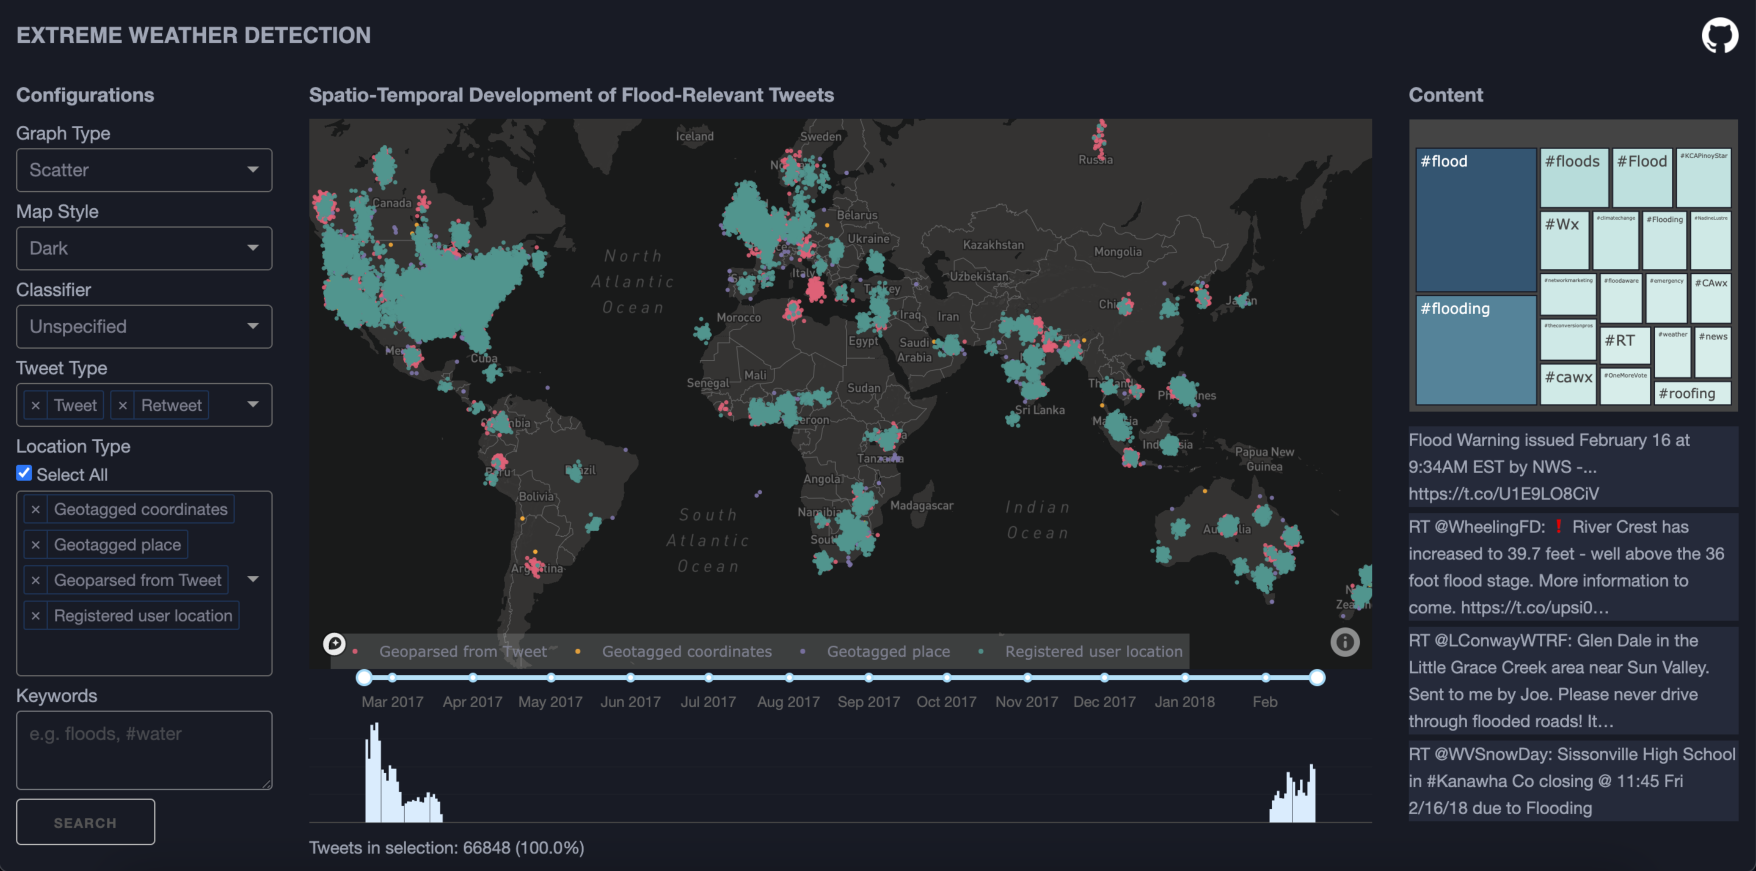
\includegraphics[width=\columnwidth]{./images/peter.png}
\end{center}
\caption{\citeauth{petersenIdentificationExplorationExtreme2021} application}
\label{fig:peter}
\end{figure}

\citeauth{fengExtractionPluvialFlood2018} use leaflet to plot a map showing flooding events as
observed in figure \ref{fig:feng}. They use $\text{Getis-Ord Gi}^{\ast}$ \cite{ordLocalSpatialAutocorrelation2010}
to detect statistical hot spots and present them as a choropleth map. The light blue circles
represent the Spatio-temporal clusters of events, and the circles with numbers at the centre
indicate clusters of tweets in that area with their total. The markers indicate individual tweets
with a pop-up containing information about it.

\begin{figure}[H]
\begin{center}
  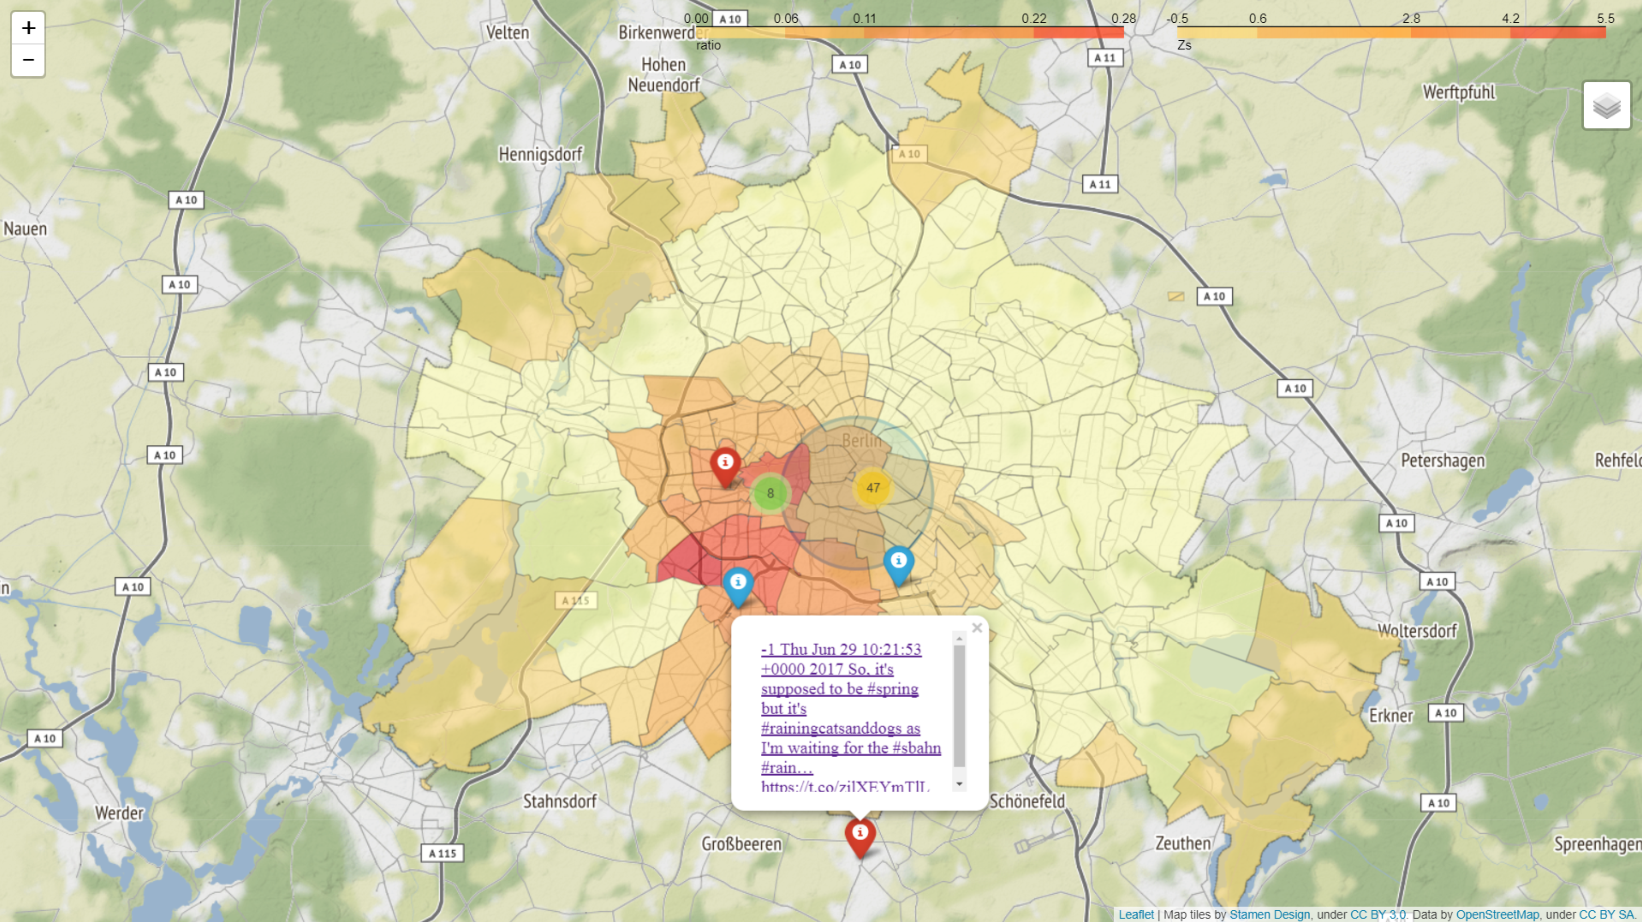
\includegraphics[width=\columnwidth]{./images/feng.png}
\end{center}
\caption{Web map application with pluvial flood in Berlin by \citeauth{fengExtractionPluvialFlood2018}}
\label{fig:feng}
\end{figure}

\citeauth{barkerDevelopmentNationalscaleRealtime2019} visualizes the tweets using different map plots
 created by leaflet. The map plot in figure \ref{fig:baker_marker} consists of clickable pointers for pop-up boxes of the tweets.

\begin{figure}[H]
\begin{center}
  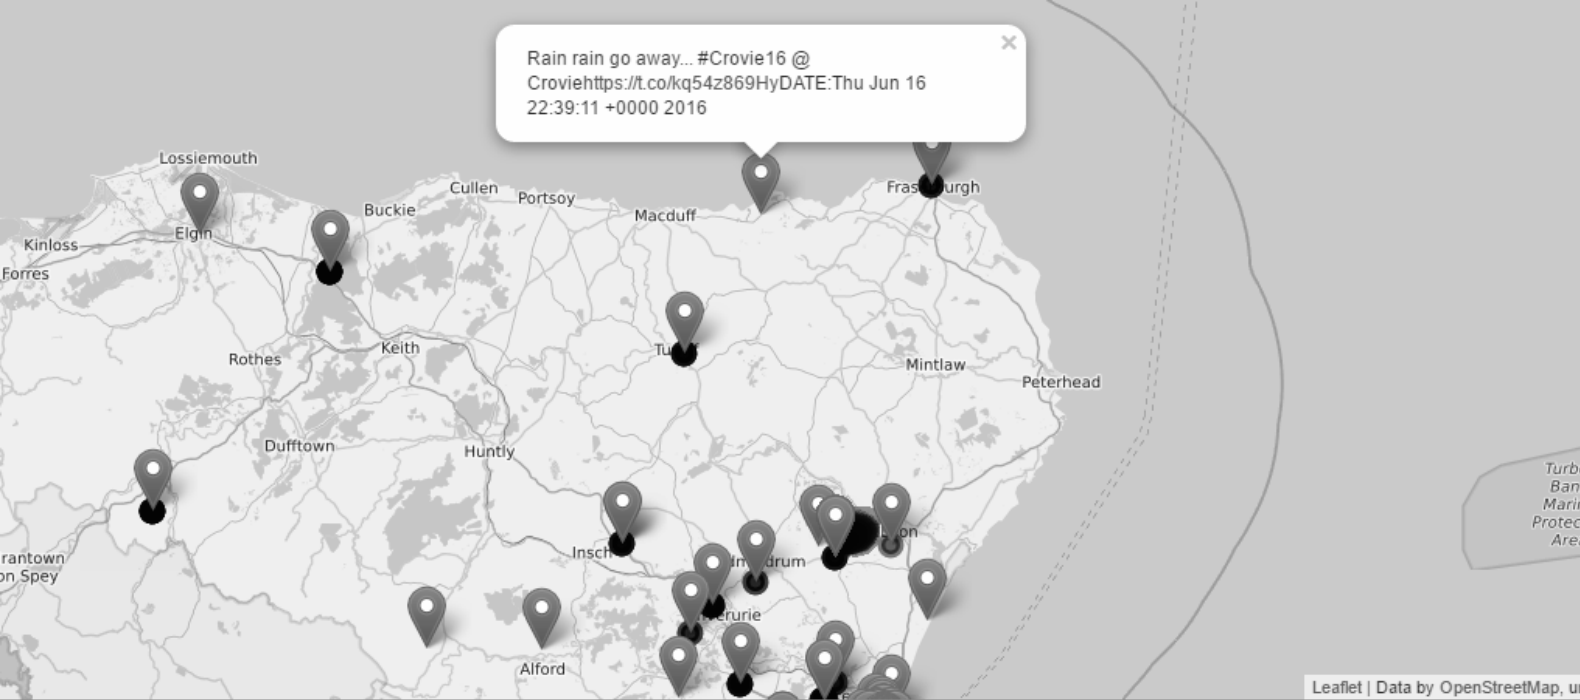
\includegraphics[width=\columnwidth]{images/baker_marker.png}
\end{center}
\caption{Map with tweet markers in by \citeauth{barkerDevelopmentNationalscaleRealtime2019}}
\label{fig:baker_marker}
\end{figure}

The bubble map in figure \ref{fig:baker_bubble} displays the tweets with the size of the circles
representing the area of the place and colour indicating the number of tweets talking about the
location.
\begin{figure}[H]
\begin{center}
  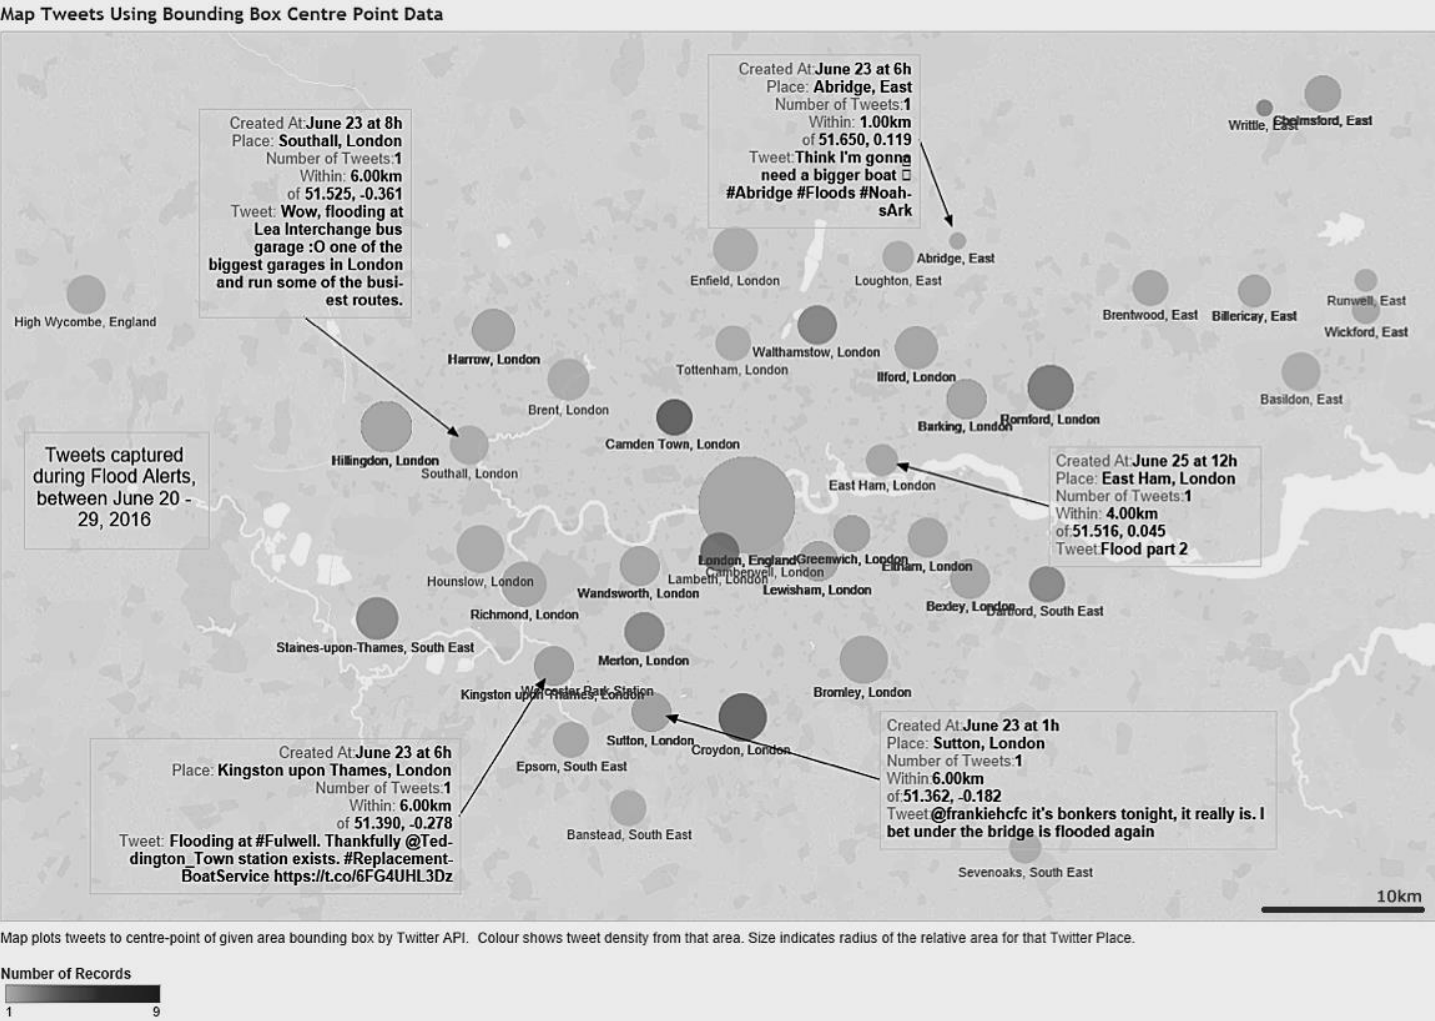
\includegraphics[width=\columnwidth]{./images/baker_bubble.png}
\end{center}
\caption{Bubble map of tweets by \citeauth{barkerDevelopmentNationalscaleRealtime2019}}
\label{fig:baker_bubble}
\end{figure}
